\documentclass{IEEEtran4PSCC}

% packages
\usepackage{lipsum}
\usepackage{ulem}
\usepackage{hyperref}
% \usepackage{flushend}
\usepackage[inline]{enumitem}
\usepackage{array,multirow,graphicx}
\usepackage{float}
\usepackage{orcidlink}

%% footnote
\usepackage{footnote}
\makesavenoteenv{tabular}
\makesavenoteenv{table}
\makesavenoteenv{tabular*}
\makesavenoteenv{table*}
% \usepackage{tablefootnote}

%% graphics packages
\usepackage{tikz}
\usepackage{colortbl}
\usepackage{pgfplots}
\usepackage{graphicx}
\usepackage{multirow}
\usepackage{multicol}
\usepackage{circuitikz}
\usepackage{dblfloatfix}
\usepackage[bottom]{footmisc}
\ifCLASSOPTIONcompsoc
    \usepackage[caption=false, font=normalsize, labelfont=sf, textfont=sf]{subfig}
\else
    \usepackage[caption=false, font=footnotesize]{subfig}
\fi

%% checkmark packages 
\usepackage{pifont}
\newcommand{\cmark}{\ding{51}}
\newcommand{\xmark}{\ding{55}}

%% math packages
\usepackage{amssymb}
\usepackage[cmex10]{amsmath}
\usepackage{mathtools}
\usepackage{booktabs}

% math 
\IEEEeqnarraydefcolsep{0}{\hoffset}
\newcommand*{\defeq}{\stackrel{\text{def}}{=}}

% definition setup
%\theoremstyle{definition}

\newtheorem{defn}{Definition}[section]

% correct bad hyphenation here
\hyphenation{op-tical net-works semi-conduc-tor}

% Set footer
\makeatletter
\let\old@ps@headings\ps@headings
\let\old@ps@IEEEtitlepagestyle\ps@IEEEtitlepagestyle
\def\psccfooter#1{%
    \def\ps@headings{%
        \old@ps@headings%
        \def\@oddfoot{\strut\hfill#1\hfill\strut}%
        \def\@evenfoot{\strut\hfill#1\hfill\strut}%
    }%
    \def\ps@IEEEtitlepagestyle{%
        \old@ps@IEEEtitlepagestyle%
        \def\@oddfoot{\strut\hfill#1\hfill\strut}%
        \def\@evenfoot{\strut\hfill#1\hfill\strut}%
    }%
    \ps@headings%
}
\makeatother

\psccfooter{%
        \parbox{\textwidth}{\hrulefill \\ \small{24th Power Systems Computation Conference} \hfill \begin{minipage}{0.2\textwidth}\centering \vspace*{4pt} 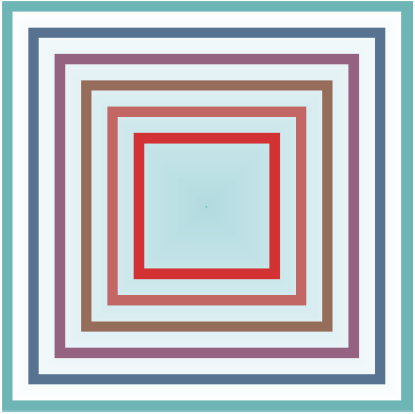
\includegraphics[scale=0.06]{PSCC_logo.png}\\\small{PSCC 2026} \end{minipage} \hfill \small{Limassol, Cyprus --- June 8 -- June 12, 2026}}%
}

\begin{document}

\onecolumn

\title{Stochastic Harmonic Hosting Capacity \\ Considering Harmonic Recombination}

\author{
\IEEEauthorblockN{Tom Van Acker\orcidlink{0000-0001-6283-1457},~Kaan Yurtseven\orcidlink{0000-0002-1384-8452},~Jinwen Xiang\orcidlink{0000-0003-2107-0238}, and Hakan Ergun\orcidlink{0000-0001-5171-1986}}
\IEEEauthorblockA{\textit{Department of Electrical Engineering} \\
\textit{KU Leuven} / \textit{EnergyVille - Etch} \\
Leuven / Genk, Belgium\\ }}

\maketitle

{\it Index terms} -- Harmonic distortion, harmonic recombination, hosting capacity, fairness, mathematical optimization.\thanksto{\noindent This work is supported by the Energy Transition Fund by FOD Economy, Belgium, project HARMONIC. The General Board on Energy of the FOD Economy is not liable for any use of the presented work and subsequent results.}

\section{Motivation}
Reaching a net zero economy by 2050 requires a massive undertaking in electrification of the energy system. In this light, over the last two decades, the number of power-electronic converters has significantly increased, both at the generation side, e.g., wind and photovoltaic generation, and at the demand side, e.g., frequency drives, electric vehicles. It is well established that one of the main downsides of power-electronic converters is their impact on the power system in terms of harmonic distortion. Sun~et~al. highlight that the traditional harmonic studies performed at the initial planning stage may no longer be appropriate~\cite{sun_distribution_2022}. Considering the transition to a heavily power-electronic dominated system, a central question to be asked is: “What is the maximum harmonic distortion, e.g., number of large-scale converters, that can be reliably hosted in a given power system?”. In literature, this concept is referred to as the hosting capacity of a power system~\cite{bollen_hosting_2017}. 

\section{Novel Contributions}
Recently, a deterministic method has been proposed to determine the lower bound on the steady-state harmonic hosting capacity of a large-scale phase-balanced three-phase power system~\cite{tom_van_acker_exact_nodate}. That paper does not consider uncertainty on the angle of the injected harmonic current, but rather assumes a constant angle relative to the reference. As such, its result is the lower bound on the steady-state harmonic hosting capacity. \textit{In this work, uncertainty on the angle of the injected harmonic current is considered, introducing the possibility for harmonic recombination to obtain a more realistic harmonic hosting capacity compared to the worst-case lower bound. To this end, probability density functions for the inherently mutually dependent harmonic angles are determined for a grid-interfacing converter based on realistic uncertainty ranges for different key topology and control parameters.} Using a fairness principle, the problem is formulated from the perspective of the power system operator, i.e., without knowledge of the (future) assets of its customers and the injected harmonic currents.

\section{The Proposed Approach}

Building on the deterministic mathematical framework presented in~\cite{tom_van_acker_exact_nodate}, the uncertainty on the angle of the injected harmonic current is modeled using polynomial chaos expansion~\cite{sullivan_introduction_2015}. Polynomial chaos expansion is a method for representing random variables in terms of polynomial functions, exhibiting superior tractability for the same accuracy compared to other stochastic modeling techniques, e.g., Monte-Carlo. In the presented method, stochastic bounds are enforced on the relevant harmonic limits, e.g., individual and total harmonic voltage distortion. Exploiting the problem structure, it becomes possible to exactly formulate the problem as a second-order cone problem, and as such the presented method remains tractable. 

\section{Numerical Experiments and Validation}

The paper presents two numerical illustrations of the stochastic harmonic hosting capacity problem of a phase-balanced three-phase power system. To this end, first, a five-bus section of a real-world industrial power system is considered to show the equivalence between the non-linear and second-order cone formulations. Second, a large-scale transmission system is
considered, to show the scalability of the proposed second-order cone formulation. 

\bibliographystyle{IEEEtran}
\bibliography{journals/dhhc/harmonic_references}

\end{document}